%% NOTES:

%\begin{Imports and headers} 
%%%%%%%%%%%%%%%%%%%%%%%%%%%%%%%%%%%%%%%%%%%%%%%%%%%%%
\documentclass[a4paper]{article}  %Or use titlepage

%% Language and font encodings
\usepackage[english]{babel}
\usepackage[utf8x]{inputenc}
\usepackage[T1]{fontenc}
\usepackage{float} %makes you be able to use H option, places fig there and only there. VERY useful

%% Sets page size and margins
\usepackage[a4paper,top=3cm,bottom=2cm,left=3cm,right=3cm,marginparwidth=1.75cm]{geometry}

%% Useful packages
\usepackage{amsmath}
\usepackage{graphicx}
\usepackage[colorinlistoftodos]{todonotes}
\usepackage[colorlinks=true, allcolors=blue]{hyperref}

%% Header, foot and page number in bottom right corner
\usepackage{fancyhdr}
\usepackage{lipsum}

%% For long comments
\usepackage{comment} 

%% For monospaced fonts
\usepackage{listings}
\lstset{
  columns=flexible,
  basicstyle=\small\ttfamily,
  mathescape=true,
  escapeinside=||
}	

% Turn on the style
\pagestyle{fancy}
% Clear the header and footer
\fancyhead{}
\fancyfoot{}
% Set the right side of the footer to be the page number
\fancyfoot[R]{\thepage}
\fancyfoot[L]{\date{\today}}
\fancyhead[C]{DD2404 - Signal peptide prediction}

%\end{Imports and headers}

\begin{document}

%\begin{Title and abstract} 
%%%%%%%%%%%%%%%%%%%%%%%%%%%%%%%%%%%%%%%%%%%%%%%%%%%%
\title{\vspace{60mm} \bf 
Signal peptide prediction}  %Fix to center title vertically
\author{Timothy Bergström}
\maketitle
\thispagestyle{fancy}  %Page number for title (\maketitle clears foot and head, so it needs to be after it)
\newpage
\tableofcontents  %OBSOBS, you need to compile the document TWO TIMES for this to work. 
\newpage

\begin{abstract}
A neural network classifier was created to predict signal peptides in proteins. The model was trained with about 1 million samples of protein sequences, which yielded a classification accuracy of 94.2\% on the test set.
The model was tested on predicting signal peptides in the Humans and Mouse proteome, which yielded 93.0\% and 93.6\% accuracy respectively in signal peptide prediction.
The model has shown that it is capable of learning general structures of signal peptides and minor improvements could be made to increase the prediction accuracy even more.

%\lipsum[1]  % Fill with nonsense
\end{abstract}
%\end{Imports and headers} 

%\begin{Introduction} 
%%%%%%%%%%%%%%%%%%%%%%%%%%%%%%%%%%%%%%%%%%%%%%%%%%%%%

\section{Introduction}


Signal peptides (SPs) are short regions in peptides that are on average between 16 to 30 amino acids long, but can be as short as 8 and as long as 65 amino acids \cite{sp_length}. SPs function is to translocate proteins to different parts of the cell, such as insertion into membranes, moving proteins to organelles or to help the cell excrete the proteins \cite{sp_wiki}. When analyzing an organisms  \href{https://en.wikipedia.org/wiki/Proteome}{proteome}, the SPs can give an indication where in the cell the proteins are translocated to, which could be of an interest when researching an organism. Not all proteins contain SPs, which is why signal peptide prediction is useful for determining the layout of the cell and for annotating organisms proteomes. 

Due to the large amount of peptide data available, manually annotating each peptide would require many man-hours, while creating and using a classifier for SPs would be more efficient.


%\end{Introduction} 

%\begin{Methods and models}
%%%%%%%%%%%%%%%%%%%%%%%%%%%%%%%%%%%%%%%%%%%%%%%%%%%%%
\section{Methods and models}

\subsection{The structure of an Signal Peptide}

SPs are located near the \href{https://en.wikipedia.org/wiki/N-terminus}{N-terminal} of a protein and have three regions; the n-region, the h-region and the c-region.

The n-region is the first region, which usually contains positively charged amino acids, making the region very polar and hydrophilic. Then comes the h-region, which contains mostly hydrophobic amino acids that forms an \href{https://en.wikipedia.org/wiki/Alpha_helix}{$\alpha$-helix} and lastly the c-region, which is usually a sequence of 3 to 8 non-charged polar amino acids. After the c-region, there is usually a cleavage site that have a tendency to be surrounded by small, uncharged amino acids.

The problem with signal peptide prediction is that polar regions in trans-membrane proteins can mistakenly be predicted as the h-region of a SP, which makes predicting SPs in trans-membrane proteins difficult.

\subsection{Design choices}
The neural network was written in python with Keras 2.0 and Tensorflow 1.4 as the backend. Keras can be used to quickly prototype and develop neural networks while the Tensorflow backend can utilize a gpu to run the calculations.

\subsection{Data sets}

A small sample of region-annotated proteins were provided by the course in \verb|fasta| format, containing mostly eukaryotic proteins. The samples also contained information if the proteins were transmembrane or not. The data set contained both positive (contains a SP) and negative samples (does not contain a SP).
Some samples was extracted from NCBI ftp server, by extracting proteins annotated with signal peptide. Few positive samples and a large set of negative samples were obtained, mostly bacterial proteins.
Many of the positive samples were scraped from Signal Peptide database. A majority of the samples were bacterial proteins.
Most samples were extracted from Swissprot protein database. Mostly eukaryotic proteins, both negative and positive.

Proteomes from Homo sapiens and Mus musculus were obtained from Swissprot, a database of high-quality manually annotated proteins \cite{swissprot}.

The training data sets were shuffled and divided in a train set, validation set and test set.

\begin{table}[H]
\centering
\begin{tabular}{l | c | c | r} %If you add more columns, change here
Database & Positive & Negative & Contains\\\hline
Swissprot & 554 196 & 573 089 & Misc eukaryotic proteins (not including Human or Mice) \\
SP database & 13 098 & 0 & Misc eukaryotic proteins (including Human and Mice) \\
Proline db & 1984 & 0 & Misc eukaryotic proteins (including Human and Mice) \\
Course data set & 1320 & 1334 & Misc proteins, from non\_TM and TM proteins \\
\end{tabular}
\caption{\label{tab:dataset_table}Training data sets}
\end{table}

\begin{table}[H]
\centering
\begin{tabular}{l | c | c | r}
Data set & Positive & Negative & From\\\hline
Human proteome & 18 807 & 144 573 & Swissprot + Ensembl \\
Mouse proteome & 10 765 & 72 675 & Swissprot + Ensembl \\
TM & 45 & 247 & Course data set \\
non\_TM & 1147 & 1087 & Course data set \\
TM + non\_TM & 1320 & 1334 & Course data set \\
\end{tabular}
\caption{\label{tab:dataset_table}Query data sets}
\end{table}

\begin{figure}[H]
\centering
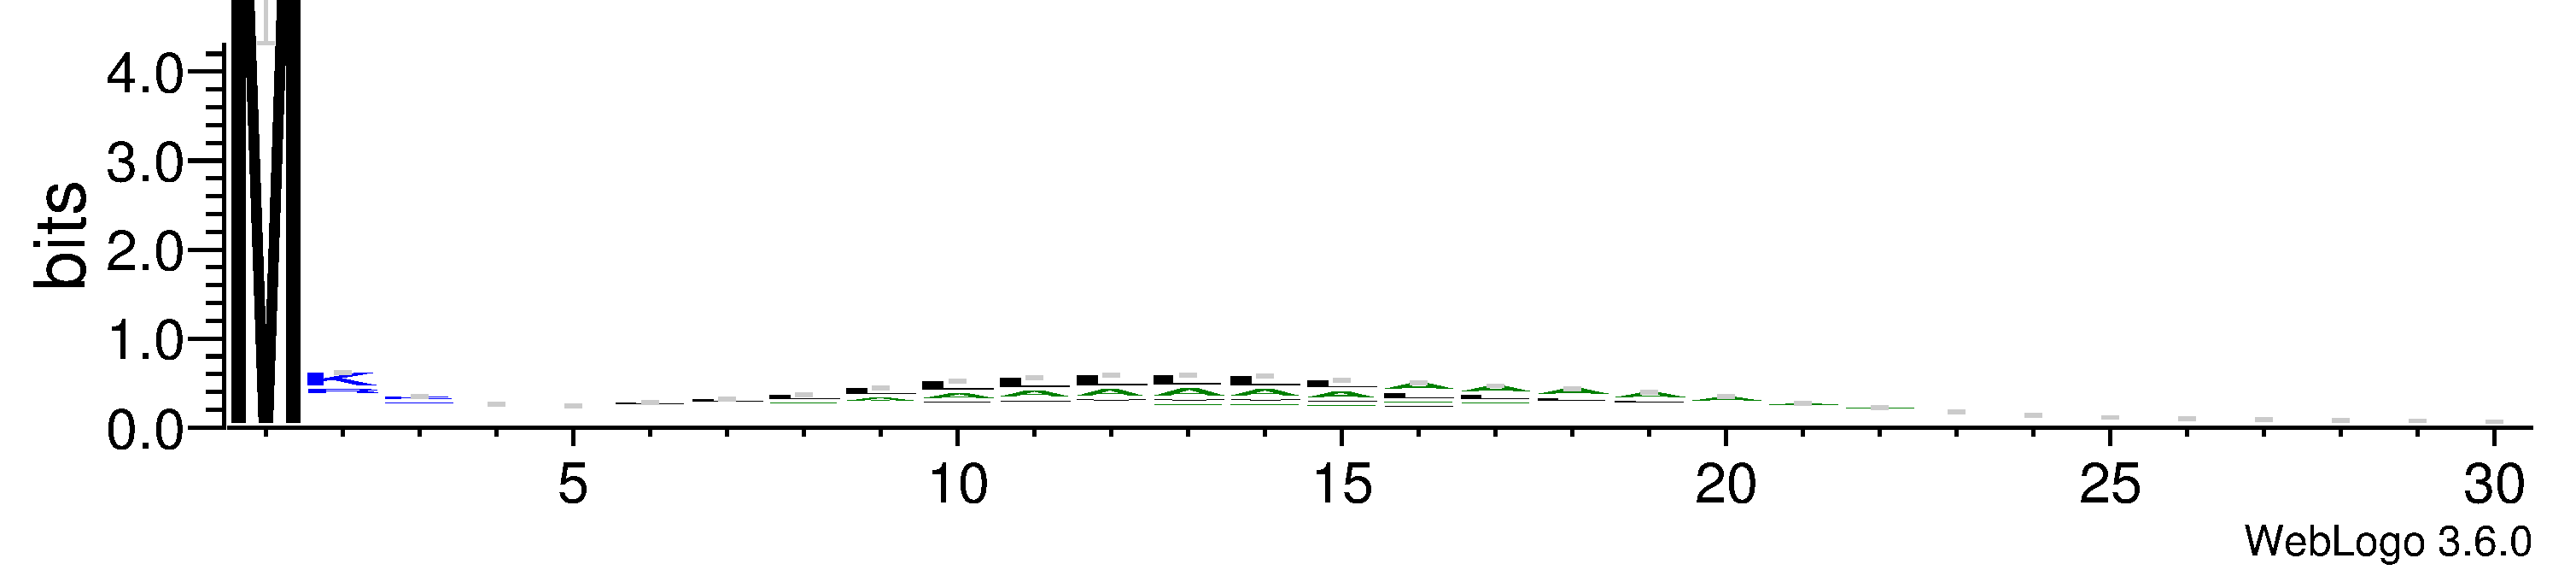
\includegraphics[width=0.7\textwidth]{pictures/train_pos_logo.png}
\caption{\label{fig:pos_seqlogo}Sequence logo of from all positive samples \cite{web_logo}}
\end{figure}

\begin{figure}[H]
\centering
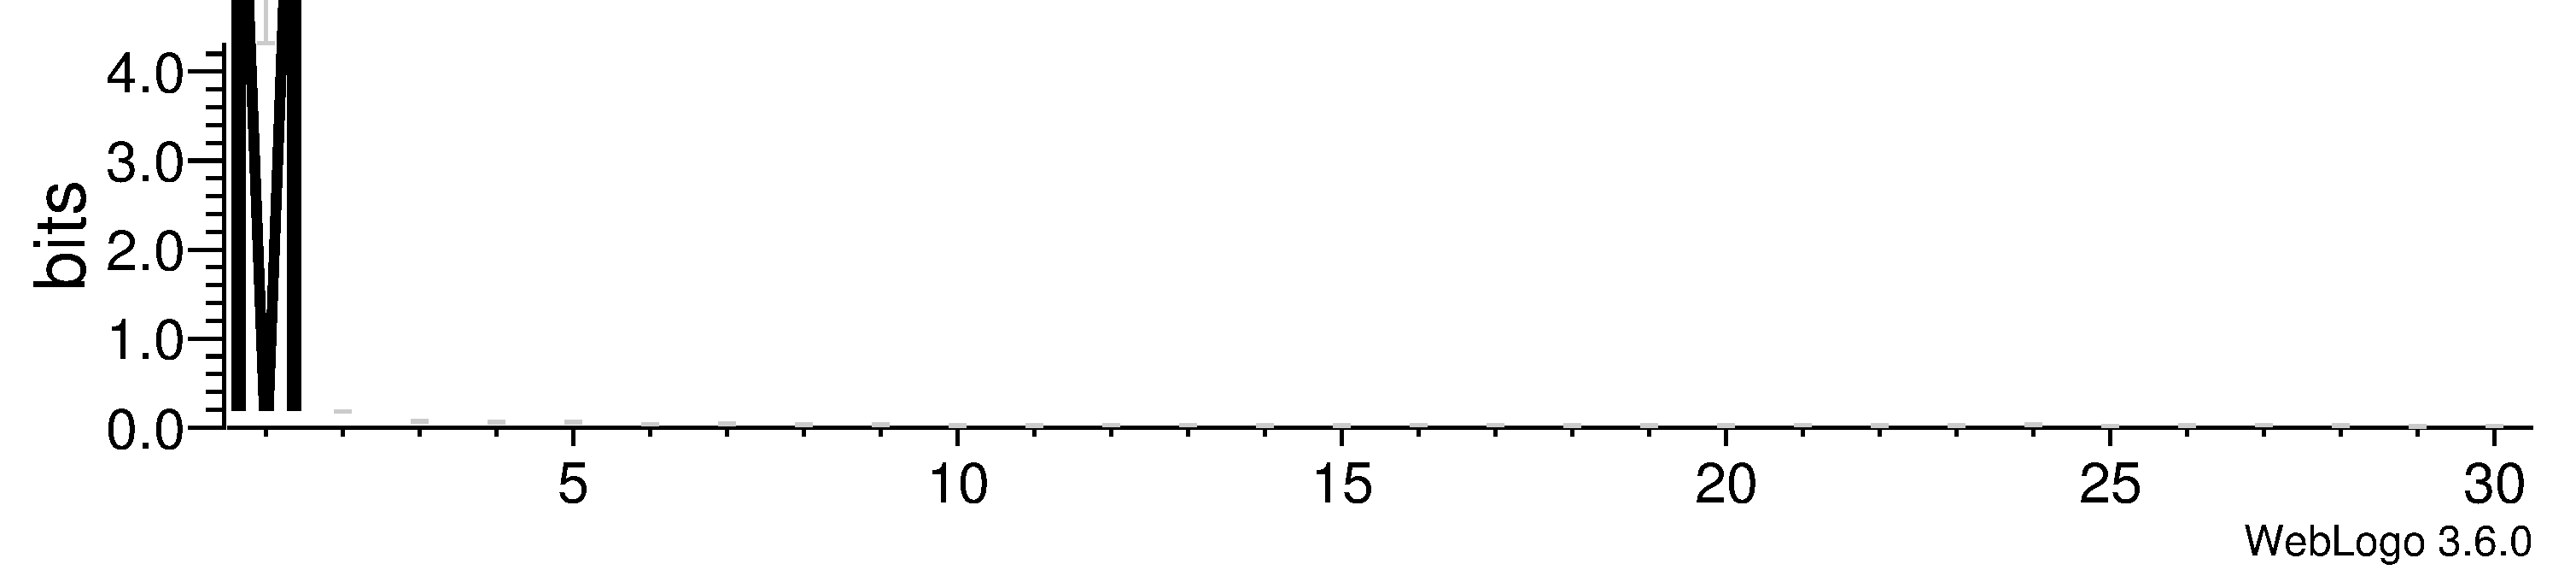
\includegraphics[width=0.7\textwidth]{pictures/train_neg_logo.png}
\caption{\label{fig:neg_seqlogo}Extracted data from all negative samples \cite{web_logo}}
\end{figure}

\subsection{Data preprocessing}

The protein sequences (samples) were contained in \verb|.fasta| files.
The first amino acid was removed, due to high bias towards some amino acids, mainly Methionine as seen in figure~\ref{fig:pos_seqlogo} and~\ref{fig:neg_seqlogo}.
The samples were then cleared from all amino acids that were not one of the 20 standard amino acids. Unknown amino acids were labeled as X.
The following 30 amino acids from each sample were used for the training data. Sequences that were too short were padded with X.
Each amino acids were then \href{https://en.wikipedia.org/wiki/One-hot}{one-hot encoded} and merged into one 2d array for each sample, creating a 3d array for all the samples. Visualization of one sample can be seen in appendix~\ref{sec:model_details}, figure~\ref{fig:sample}.
Negative samples were labeled as 0 and positive samples were labeled as 1.
The data was lastly \href{https://en.wikipedia.org/wiki/Oversampling_and_undersampling_in_data_analysis}{undersampled}, making the ratio between negative and positive samples 50/50 to prevent overfittning.

\subsection{Neural Network structure}
The neural network was based on bidirectional \href{http://colah.github.io/posts/2015-08-Understanding-LSTMs/}{LSTMs}, due to LSTMs effectiveness with sequences and pattern recognition \cite{rnn_effectiveness}. The bidirectionality of the network was added due to its success in other areas of machine learning with sequences and time-series predictions \cite{bidirectional_1} \cite{bidirectional_2}. The input was one 2d array and the output was one float, ranging from 0 to 1. A regularization layer was added between the LSTM layers to prevent overfitting.

\begin{figure}[H]
\centering
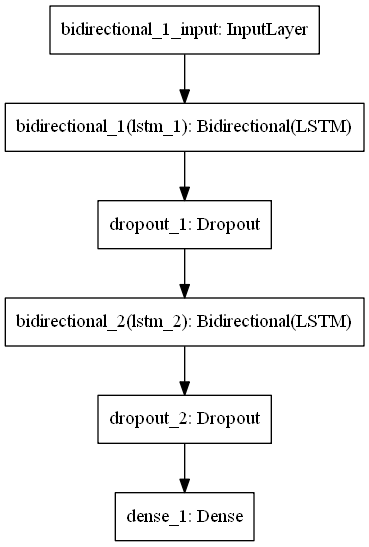
\includegraphics[width=0.4\textwidth]{pictures/model.png}
\caption{\label{fig:model_fig}Prediction model}
\end{figure}


\subsection{Related works}

There are multiple softwares and websites that predicts signal peptides, such as SignalP, SignalBlast and Predisi to name a few \cite{sp_predict1} \cite{sp_predict2} \cite{sp_predict3}. Neural Networks (NN) are the most used methods while some sites use Hidden Markov Models (HMM) instead. Similar methods can used to predict other biological problems, such as motifs and trans-membrane regions in proteins.

%\end{Methods and models}

%\begin{Evaluating model}
%%%%%%%%%%%%%%%%%%%%%%%%%%%%%%%%%%%%%%%%%%%%%%%%%%%%%
\section{Evaluating model}

\subsection{Model performance}

The model performed very well and showed no signs of overfitting during training, which can be seen in figure~\ref{fig:train_loss}. A model that has overfitted can be seen in figure~\ref{fig:overfit} in appendix~\ref{sec:pitfalls}.

\begin{figure}[H]
\center
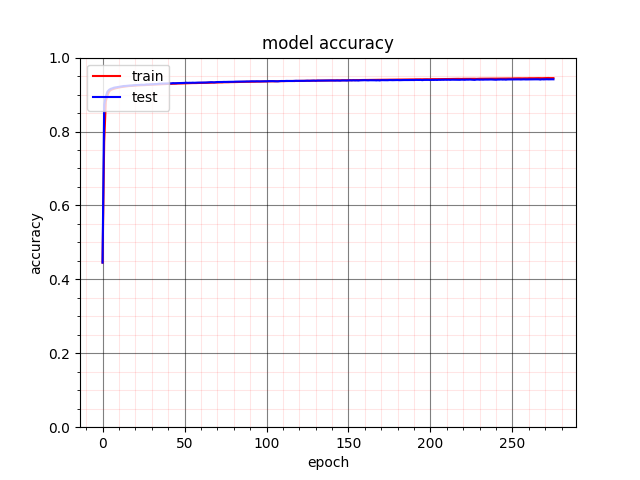
\includegraphics[width=0.7\textwidth]{pictures/train_acc.png}
\caption{\label{fig:train_acc}Model accuracy during training}
\end{figure}

\begin{figure}[H]
\center
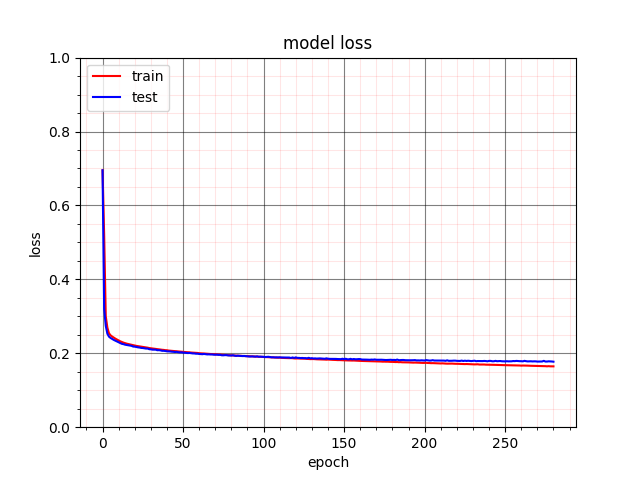
\includegraphics[width=0.7\textwidth]{pictures/train_loss.png}
\caption{\label{fig:train_loss}Model loss during training}
\end{figure}

\begin{figure}[H]
\center
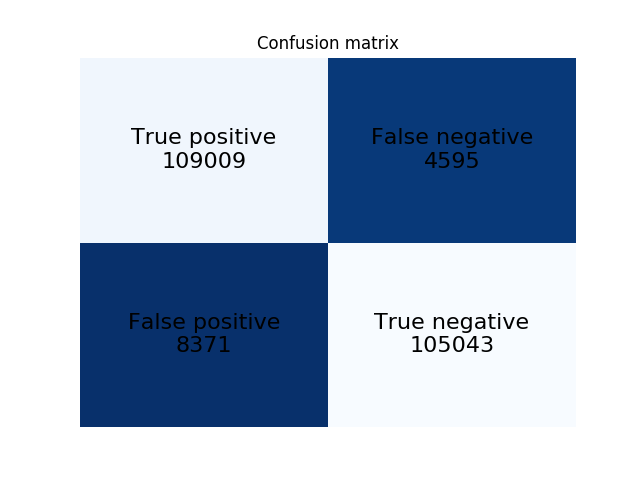
\includegraphics[width=0.7\textwidth]{pictures/train_cm.png}
\caption{\label{fig:train_cm}Confusion matrix on test set after training}
\end{figure}

\begin{figure}[H]
\center
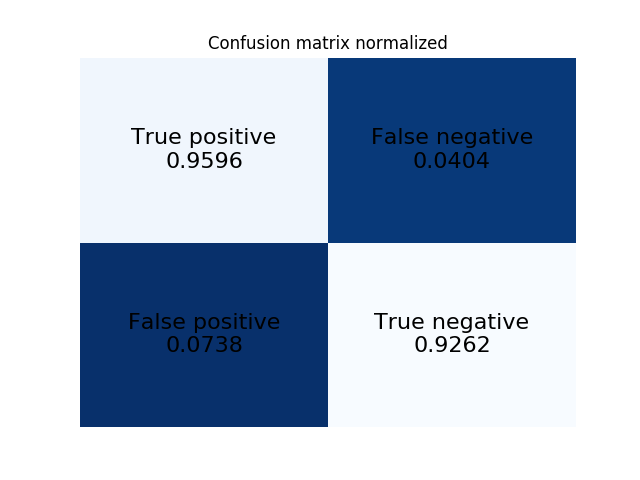
\includegraphics[width=0.7\textwidth]{pictures/train_cm_normalized.png}
\caption{\label{fig:train_normalized_cm}Normalized confusion matrix on test set after training}
\end{figure}

\begin{figure}[H]
\center
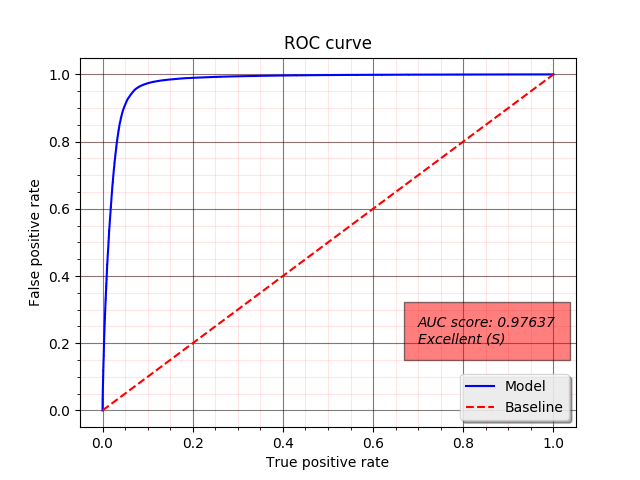
\includegraphics[width=0.7\textwidth]{pictures/train_roc.png}
\caption{\label{fig:train_roc}ROC curve on test set after training}
\end{figure}

\begin{table}[H]
\centering
\begin{tabular}{l | r} %If you add more columns, change here
Statistical value & value\\\hline
Accuracy & 0.9429 \\
Precision & 0.9287 \\
Sensitivity & 0.9596 \\
Specificity & 0.9262 \\
\end{tabular}
\caption{\label{tab:stat_table}Statistical values: Training}
\end{table}

\subsection{Signal peptide detection in transmembrane proteins}

\subsubsection{Non TM proteins}

The model performed better with non TM proteins than with the training data set. All statistical values are high, showing no signs of overfitting to the data.

\begin{figure}[H]
\center
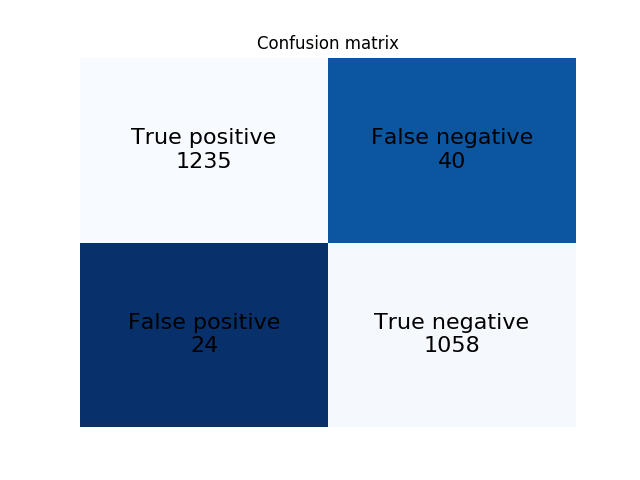
\includegraphics[width=0.7\textwidth]{pictures/non_tm_cm.png}
\caption{\label{fig:non_tm_cm}Confusion matrix on non TM proteins}
\end{figure}

\begin{figure}[H]
\center
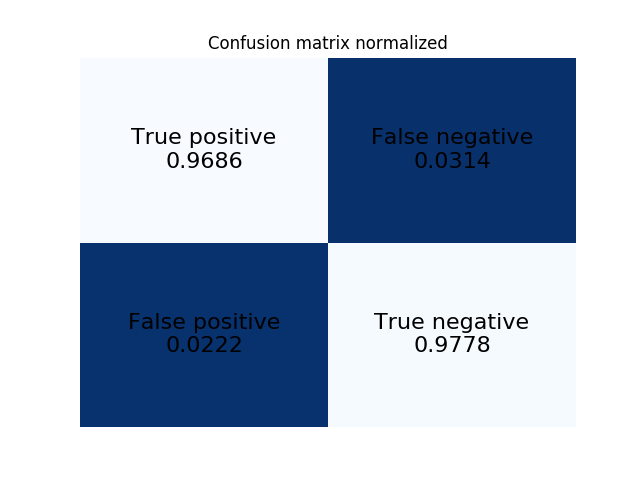
\includegraphics[width=0.7\textwidth]{pictures/non_tm_cm_normalized.png}
\caption{\label{fig:non_tm_normalized_cm}Normalized confusion matrix on non TM proteins}
\end{figure}

\begin{figure}[H]
\center
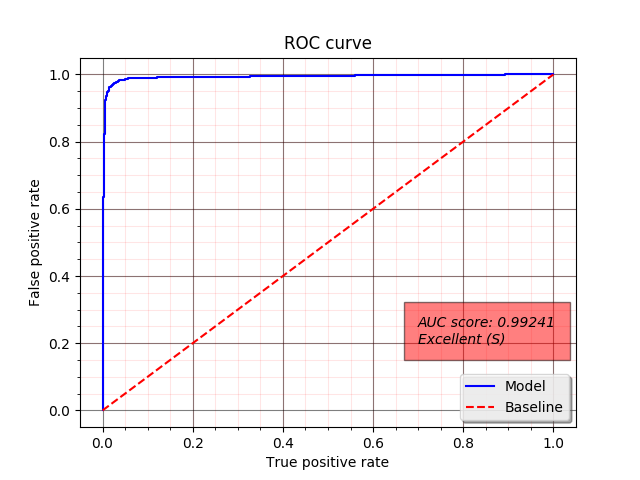
\includegraphics[width=0.7\textwidth]{pictures/non_tm_roc.png}
\caption{\label{fig:non_tm_roc}ROC curve on non TM proteins}
\end{figure}

\begin{table}[H]
\centering
\begin{tabular}{l | r} %If you add more columns, change here
Statistical value & value\\\hline
Accuracy & 0.9728 \\
Precision & 0.9809 \\
Sensitivity & 0.9686 \\
Specificity & 0.9778 \\
\end{tabular}
\caption{\label{tab:non_tm_stat_table}Statistical values: non TM proteins}
\end{table}


\subsubsection{TM proteins}

The precision is rather low compared to non TM, but it still has an acceptable prediction peformance.

\begin{figure}[H]
\center
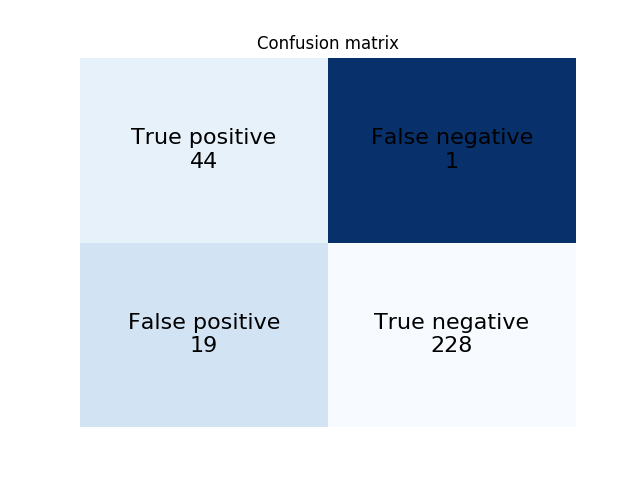
\includegraphics[width=0.7\textwidth]{pictures/tm_cm.png}
\caption{\label{fig:tm_cm}Confusion matrix on TM proteins}
\end{figure}

\begin{figure}[H]
\center
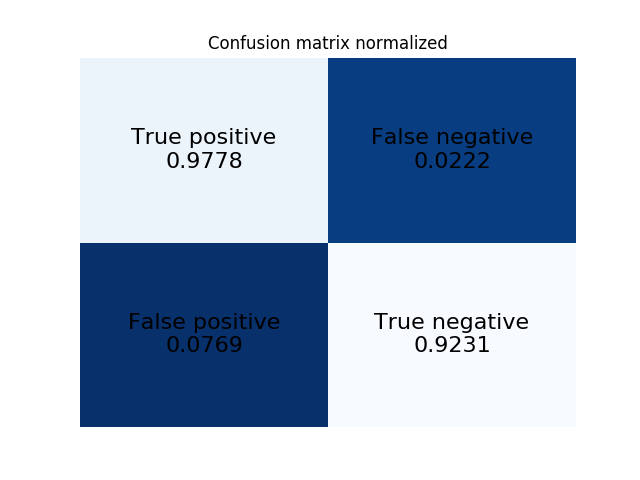
\includegraphics[width=0.7\textwidth]{pictures/tm_cm_normalized.png}
\caption{\label{fig:tm_normalized_cm}Normalized confusion matrix on TM proteins}
\end{figure}

\begin{figure}[H]
\center
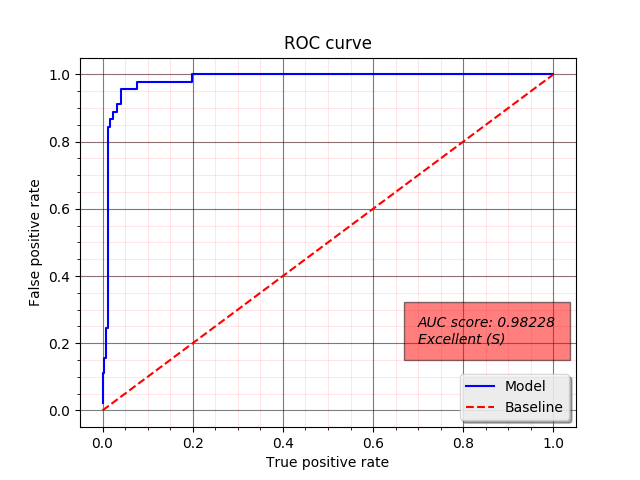
\includegraphics[width=0.7\textwidth]{pictures/tm_roc.png}
\caption{\label{fig:tm_roc}ROC curve on TM proteins}
\end{figure}

\begin{table}[H]
\centering
\begin{tabular}{l | r} %If you add more columns, change here
Statistical value & value\\\hline
Accuracy & 0.9315 \\
Precision & 0.6984 \\
Sensitivity &  0.9778 \\
Specificity & 0.9231 \\
\end{tabular}
\caption{\label{tab:tm_stat_table}Statistical values: TM proteins}
\end{table}


\subsection{Signal peptide detection in proteomes}

\subsubsection{Human proteome}

As the TM proteins, the precision is rather low compared to the training data set and the non TM data set.

\begin{figure}[H]
\center
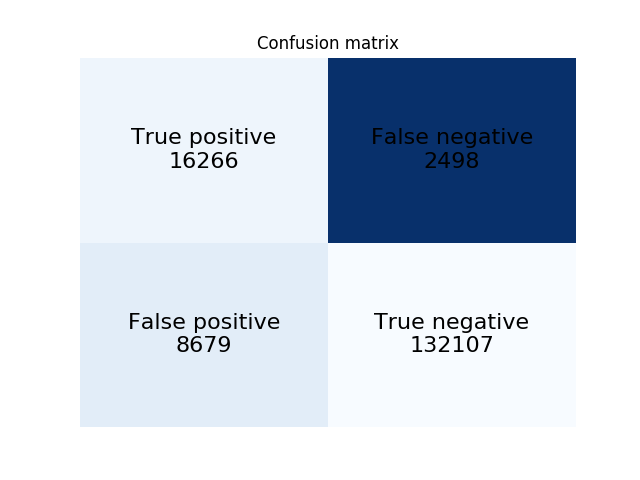
\includegraphics[width=0.7\textwidth]{pictures/human_cm.png}
\caption{\label{fig:human_cm}Confusion matrix on human proteome}
\end{figure}

\begin{figure}[H]
\center
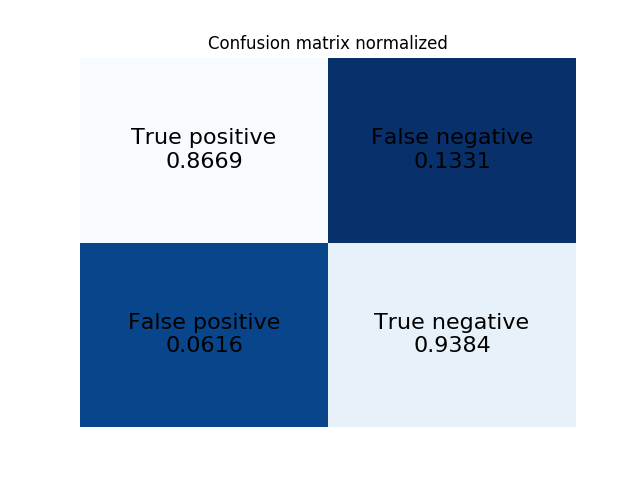
\includegraphics[width=0.7\textwidth]{pictures/human_cm_normalized.png}
\caption{\label{fig:human_normalized_cm}Normalized confusion matrix on human proteome}
\end{figure}

\begin{figure}[H]
\center
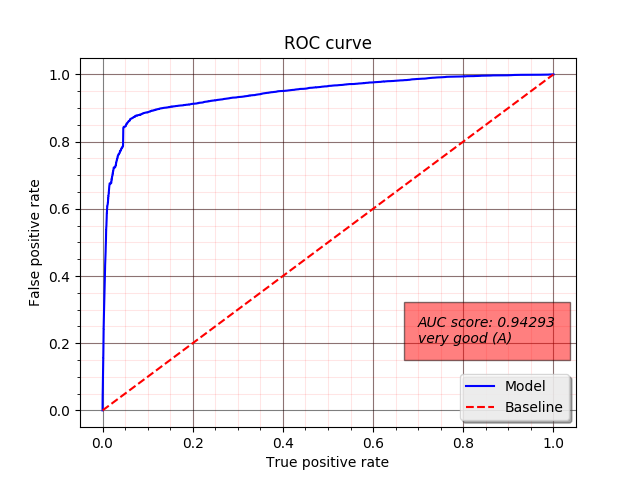
\includegraphics[width=0.7\textwidth]{pictures/human_roc.png}
\caption{\label{fig:human_roc}ROC curve on human proteome}
\end{figure}

\begin{table}[H]
\centering
\begin{tabular}{l | r} %If you add more columns, change here
Statistical value & value\\\hline
Accuracy & 0.9299 \\
Precision & 0.6521 \\
Sensitivity & 0.8669 \\
Specificity & 0.9384 \\
\end{tabular}
\caption{\label{tab:human_stat_table}Statistical values: Human}
\end{table}

\subsubsection{Mouse proteome}

Precision is higher than the Human proteome, but still rather low.

\begin{figure}[H]
\center
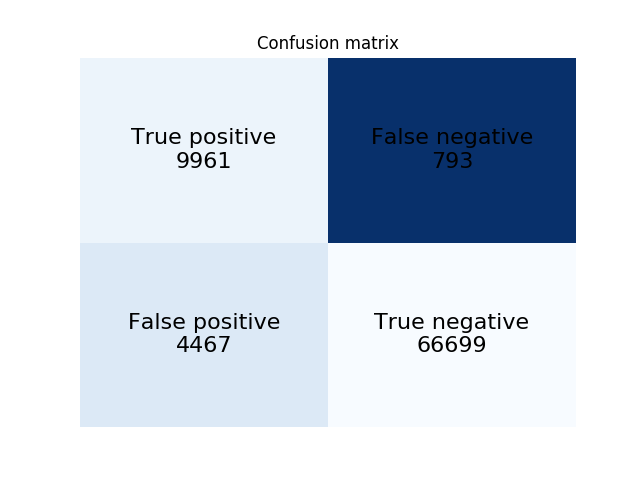
\includegraphics[width=0.7\textwidth]{pictures/mouse_cm.png}
\caption{\label{fig:mouse_cm}Confusion matrix on mouse proteome}
\end{figure}

\begin{figure}[H]
\center
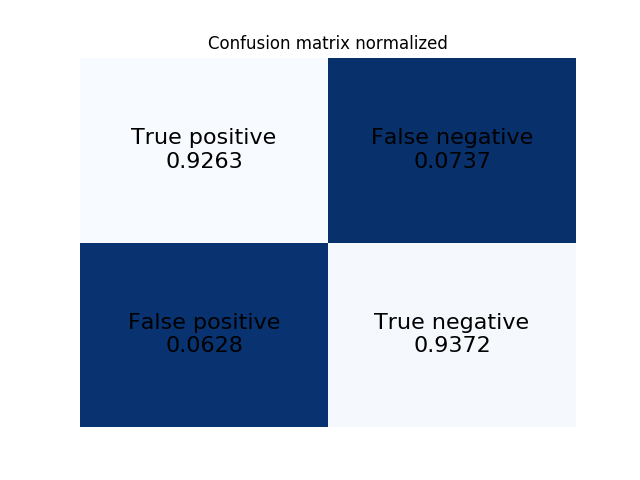
\includegraphics[width=0.7\textwidth]{pictures/mouse_cm_normalized.png}
\caption{\label{fig:mouse_normalized_cm}Normalized confusion matrix on mouse proteome}
\end{figure}

\begin{figure}[H]
\center
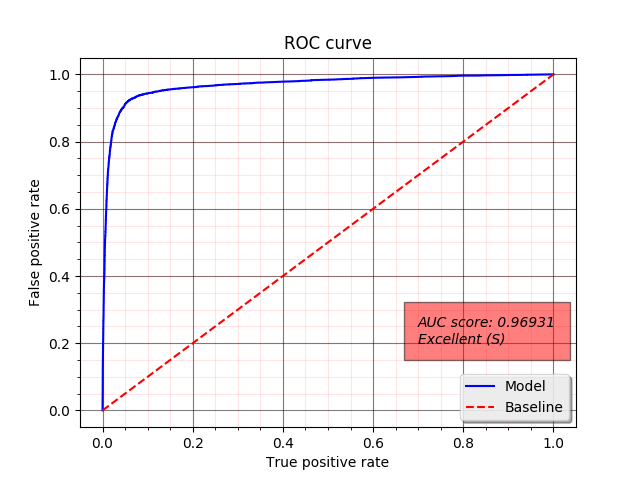
\includegraphics[width=0.7\textwidth]{pictures/mouse_roc.png}
\caption{\label{fig:mouse_roc}ROC curve on mouse proteome}
\end{figure}

\begin{table}[H]
\centering
\begin{tabular}{l | r} %If you add more columns, change here
Statistical value & value\\\hline
Accuracy & 0.9358 \\
Precision & 0.6904 \\
Sensitivity & 0.9263 \\
Specificity & 0.9372 \\
\end{tabular}
\caption{\label{tab:mouse_stat_table}Statistical values: Mouse}
\end{table}

%\end{Evaluating model}

%\begin{Conclusion}
%%%%%%%%%%%%%%%%%%%%%%%%%%%%%%%%%%%%%%%%%%%%%%%%%%%%%
\section{Conclusion}

{\em Why are the precisions low for TM proteins and the proteomes compared to the training data set and non TM proteins?}

One reason could be that there are very few positive samples in the data sets compared to the amount of negative samples. Precision is calculated with the equation:
\newline

\begin{equation}
	precision = \dfrac{TP}{FP+TP}
\end{equation}
\newline

The equation shows that a high amount of false positives (negative data predicted as positive) will decrease the precision, while in table~\ref{tab:dataset_table} it can be seen the amount of positives are much lower than the amount of negatives for the data sets, about 5.5 times more negative samples than positive for TM proteins.

Another reason for the discrepancy could be that the training data mostly contained non TM proteins and that it is bad at predicting TM proteins. It might also be that a majority of the proteomes are TM proteins.
\newline

{\em How does the model compare to other models on the web?}

Comparing the model to PrediSi and SignalP, the created model is superior in accuracy for positive eukarytic proteins, while the created model has an inferior accuracy for negative samples as shown in table~\ref{tab:other_models_table}. However, you have to take into account that PrediSi and  SignalP also tries to predict cleavage sites and other regions in proteins, while the created model simply predict if the proteins contain signal peptides or not.

\begin{table}[H]
\centering
\begin{tabular}{l | r | r}
Website & Positive accuracy & Control accuracy\\\hline
PrediSi & 72.66 & 98.30\\
SignalP (NN) & 82.11 & 99.21\\
SignalP (HMM) & 78.73 & 97.74\\
\end{tabular}
\caption{\label{tab:other_models_table}Other models and accuracies for eukarytoic proteins \cite{other_websites}}
\end{table}


In conclusion; The neural network is a good prediction model that has shown potential. Improvements can be made, such as higher quality data for training, a larger architecture and longer training times. The model could potentially be used for other applications, such as predicting exons in DNA or other areas, such as text or speech recognition.
\newline

All the source code can be found on github:

\url{https://github.com/TimothyBergstrom/DD2404-project}


%\end{Conclusion}

%\begin{References}
%%%%%%%%%%%%%%%%%%%%%%%%%%%%%%%%%%%%%%%%%%%%%%%%%%%%%
\newpage
%% References
\bibliographystyle{alpha}
\begin{thebibliography}{9}

\bibitem{sp_length} Henrik Nielsen, {\em SignalP V1.1 World Wide Web Prediction Server}
\url{http://www.cbs.dtu.dk/services/SignalP-1.1/sp_lengths.html}

\bibitem{sp_wiki} Wikipedia, {\em Signal peptides wikipedia}
\url{https://en.wikipedia.org/wiki/Signal_peptide}

\bibitem{swissprot} The UniProt Consortium
UniProt: the universal protein knowledgebase
Nucleic Acids Res. 45: D158-D169 (2017), {\em Swissprot database}
\url{http://www.uniprot.org/uniprot/?query=reviewed:yes}

\bibitem{web_logo} Crooks GE, Hon G, Chandonia JM, Brenner SE WebLogo: A sequence logo generator, Genome Research, 14:1188-1190, (2004)
Schneider TD, Stephens RM. 1990.{\em Sequence Logos: A New Way to Display Consensus Sequences} Nucleic Acids Res. 18:6097-6100

\bibitem{rnn_effectiveness} Karpathy, {\em The Unreasonable Effectiveness of Recurrent Neural Networks}
May 21, 2015
\url{http://karpathy.github.io/2015/05/21/rnn-effectiveness/}

\bibitem{bidirectional_1} Ankita Sharma, Yokila Arora, {\em Sequential LSTM-based Encoder for NLI}
\url{https://web.stanford.edu/class/cs224n/reports/2760320.pdf}

\bibitem{bidirectional_2} Zhou Yu et al, {\em USING BIDIRECTIONAL LSTM RECURRENT NEURAL NETWORKS TO LEARN HIGH-LEVEL ABSTRACTIONS OF SEQUENTIAL FEATURES FOR AUTOMATED SCORING OF NON-NATIVE SPONTANEOUS SPEECH}
\url{http://www.cs.cmu.edu/afs/cs/user/zhouyu/www/ASRU.pdf}

\bibitem{sp_predict1} Henrik Nielsen,
{\em Predicting Secretory Proteins with SignalP},
In Kihara, D (ed): Protein Function Prediction (Methods in Molecular Biology vol. 1611),  pp. 59-73, Springer 2017, doi: 10.1007/978-1-4939-7015-5\_6, PMID: 28451972, 
\url{http://www.cbs.dtu.dk/services/SignalP/}  %CHAR _ makes Latex crash, use \_

\bibitem{sp_predict2} Karl Frank; Manfred J. Sippl,
{\em High Performance Signal Peptide Prediction Based on Sequence Alignment Techniques},
Bioinformatics, 24, pp. 2172-2176 (2008), \url{http://sigpep.services.came.sbg.ac.at/signalblast.html}

\bibitem{sp_predict3}  Karsten Hiller,
{\em PrediSi}, Institute for Microbiology Technical University of Braunschweig, 
\url{http://www.predisi.de/}

\bibitem{other_websites} Karsten Hiller  Andreas Grote, Maurice Scheer, Richard Münch, Dieter Jahn, {\em PrediSi: prediction of signal peptides and their cleavage positions}
Nucleic Acids Research, Volume 32, Issue suppl\_2, 1 July 2004, Pages W375–W379
Published: 01 July 2004

\url{https://academic.oup.com/nar/article/32/suppl_2/W375/1040487}

\end{thebibliography}

%\end{References}

%\begin{Appendix}
%%%%%%%%%%%%%%%%%%%%%%%%%%%%%%%%%%%%%%%%%%%%%%%%%%%%%
\newpage

\section{Appendix}

\subsection{Model details}\label{sec:model_details}

\begin{lstlisting}
_________________________________________________________________
Layer (type)                      Output Shape         Param #   
=================================================================
bidirectional_1 (Bidirection     (None, 30, 128)       44032     
_________________________________________________________________
dropout_1 (Dropout)              (None, 30, 128)       0         
_________________________________________________________________
bidirectional_2 (Bidirection     (None, 128)           98816     
_________________________________________________________________
dropout_2 (Dropout)              (None, 128)           0         
_________________________________________________________________
dense_1 (Dense)                  (None, 1)             129       
=================================================================
Total params: 142,977
Trainable params: 142,977
Non-trainable params: 0
_________________________________________________________________
Input shape: (None, 30, 21)
Output shape: (None, 1)

\end{lstlisting}

Train set: 362 844 positive samples and 363 615 negative samples

Validation set: 91 098 positive samples and 90 517 negative samples

Test set: 113 604 positive samples and 113 414 negative samples
\newline

12 hours trained with on a GTX 970.
Batch size of 4096, dropout of 0.5 for each layer and using ADAM optimizer with default learning rate 0.0001.
\newline  % bug here after using plaintext, this fixes it

The input data was a batch of (30, 21) arrays, corresponding to 30 amino acid long sequences with 21 possible amino acids (20 standard amino acids + unknown acid X).

\begin{figure}[H]
\center
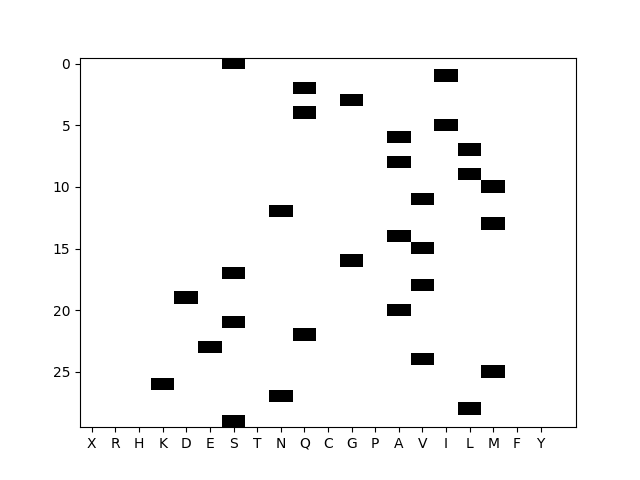
\includegraphics[width=0.7\textwidth]{pictures/sample.png}
\caption{\label{fig:sample}Visualization of sample after one-hot encoding}
\end{figure}


\subsection{Pitfalls when training a model}\label{sec:pitfalls}
Examples of overfitting and other problems that you will encounter when training a neural network.

\begin{figure}[H] %Rank in order
\center
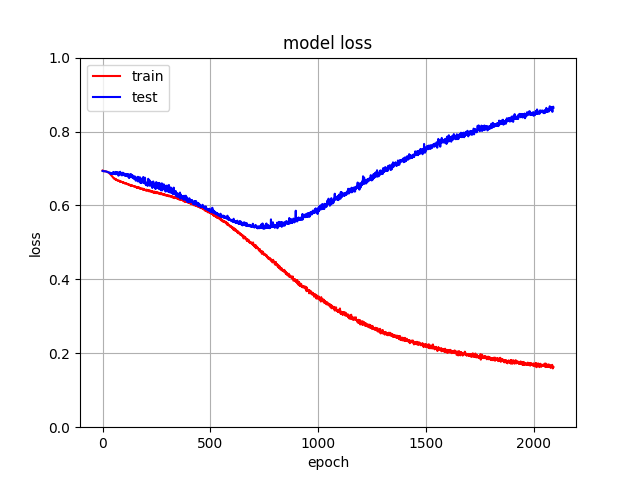
\includegraphics[width=0.7\textwidth]{pictures/overfit.png}
\caption{\label{fig:overfit}Overfitted}
\end{figure}

\begin{figure}[H]
\center
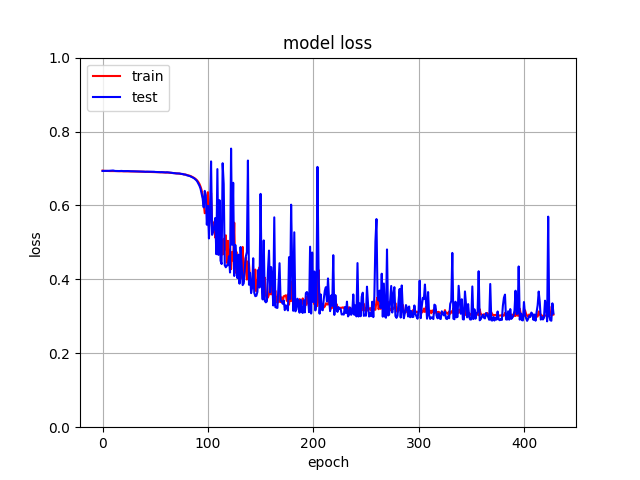
\includegraphics[width=0.7\textwidth]{pictures/high_lr.png}
\caption{\label{fig:high_lr}Too high learning rate}
\end{figure}

\begin{figure}[H]
\center
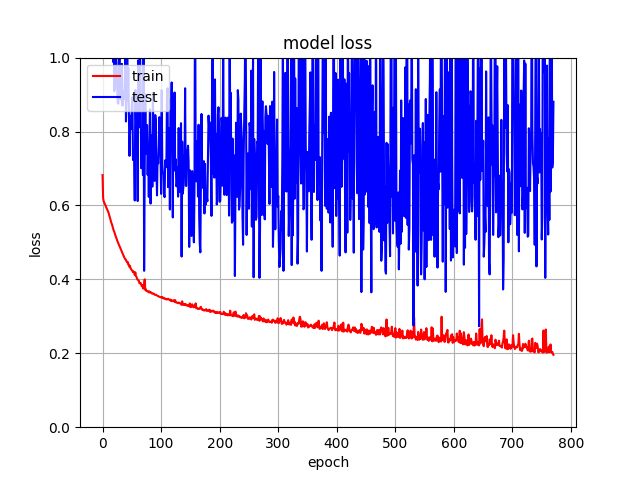
\includegraphics[width=0.7\textwidth]{pictures/no_shuffle.png}
\caption{\label{fig:no_shuffle}Data not shuffled}
\end{figure}


\begin{comment}
\subsection{Additional features}


List of things
\begin{enumerate}
\item Data augmentation,
\item Data conversion
\end{enumerate}

The data can be loaded in many ways. One way is to augment the data by dividing each sequence into many chunks, labeling the chunk closest to the N-terminal as positive and the rest as negative.

Due to the large amount of data obtained, data augmentation were not used.
\linebreak

Advantages with data augmentation:
\begin{itemize}
\item Each positive sample would yield multiple negative samples, so smaller data sets can be used for training.
\item Using positive samples and the negative samples from different organisms could make the model overfit to a particular amino acid bias. Using other regions of the positive samples would preserve the amino acid bias, making the data more consistent.
\item Some trans-membrane regions of the proteins might be very similar to signal peptide regions, which would force the model to improve the prediction of trans-membrane proteins. 
\end{itemize}

Disadvantages with data augmentation:
\begin{itemize}
\item The first amino acid in the N-terminal has an high bias towards some amino acids, mainly Methionine, see Figure~\ref{fig:pos_seqlogo}. The model would then have a high affinity for the first amino acids, creating a poor model that would only detect if the sequence is located in the N-terminal or not. The first amino acids of each sequence were removed, preventing the problem if data augmentation were to be used.
\item The N-terminal of peptides both with and without SPs might have a similar structure compared to other regions of protein, which would make the model as stated above, only be able to distinguish if the region is at the N-terminal or not. To prevent this problem, using both negative samples from N-regions and other regions should be used.
\end{itemize}
\end{comment}


%\end{Appendix}

\end{document}
